% ============================================================
% Question Bank: ch04-05 Adding and Subtracting Linear Expressions
% Topic Title: Adding and Subtracting Linear Expressions
% CCSS: 7.EE.A.1
% Questions: 27 (15 MC + 6 SA + 6 Graphical)
% ============================================================

% --- Multiple Choice Questions (15) ---

\begin{practiceQuestion}{4-5-q01}{mc}
\begin{questionText}
Simplify $(4x + 7) + (3x + 2)$.
\end{questionText}
\choiceA{$7x + 9$}
\choiceB{$7x + 5$}
\choiceC{$12x + 9$}
\choiceD{$7x - 9$}
\correctAnswer{A}
\explanation{Combine like terms: $4x + 3x = 7x$ and $7 + 2 = 9$. Result: $7x + 9$.}
\end{practiceQuestion}

\begin{practiceQuestion}{4-5-q02}{mc}
\begin{questionText}
Simplify $(8a - 3) - (2a + 5)$.
\end{questionText}
\choiceA{$6a + 2$}
\choiceB{$6a - 8$}
\choiceC{$10a - 8$}
\choiceD{$6a + 8$}
\correctAnswer{B}
\explanation{Distribute the negative: $8a - 3 - 2a - 5$. Combine: $8a - 2a = 6a$ and $-3 - 5 = -8$. Result: $6a - 8$.}
\end{practiceQuestion}

\begin{practiceQuestion}{4-5-q03}{mc}
\begin{questionText}
What is $(5n + 4) + (-2n + 9)$?
\end{questionText}
\choiceA{$3n + 13$}
\choiceB{$7n + 13$}
\choiceC{$3n - 5$}
\choiceD{$3n + 5$}
\correctAnswer{A}
\explanation{Combine: $5n + (-2n) = 3n$ and $4 + 9 = 13$. Result: $3n + 13$.}
\end{practiceQuestion}

\begin{practiceQuestion}{4-5-q04}{mc}
\begin{questionText}
Simplify $(9y - 6) - (4y - 1)$.
\end{questionText}
\choiceA{$5y - 7$}
\choiceB{$5y - 5$}
\choiceC{$13y - 7$}
\choiceD{$5y + 5$}
\correctAnswer{B}
\explanation{Distribute the negative: $9y - 6 - 4y + 1$. Combine: $9y - 4y = 5y$ and $-6 + 1 = -5$. Result: $5y - 5$.}
\end{practiceQuestion}

\begin{practiceQuestion}{4-5-q05}{mc}
\begin{questionText}
A student simplifies $(7x + 3) - (2x + 8)$ as $5x + 11$. What mistake did the student make?
\end{questionText}
\choiceA{Added the $x$-terms instead of subtracting}
\choiceB{Did not distribute the negative sign to $+8$}
\choiceC{Reversed the order of the terms}
\choiceD{Added both constants instead of subtracting}
\correctAnswer{B}
\explanation{The student correctly got $5x$ but then added $3 + 8 = 11$ instead of subtracting $3 - 8 = -5$. The negative sign must be distributed to both terms in the second expression. Correct answer: $5x - 5$.}
\end{practiceQuestion}

\begin{practiceQuestion}{4-5-q06}{mc}
\begin{questionText}
Add $(3.5x - 2.1) + (1.5x + 4.6)$.
\end{questionText}
\choiceA{$5x + 2.5$}
\choiceB{$5x - 6.7$}
\choiceC{$2x + 2.5$}
\choiceD{$5x + 6.7$}
\correctAnswer{A}
\explanation{Combine: $3.5x + 1.5x = 5x$ and $-2.1 + 4.6 = 2.5$. Result: $5x + 2.5$.}
\end{practiceQuestion}

\begin{practiceQuestion}{4-5-q07}{mc}
\begin{questionText}
Simplify $\left(\frac{2}{3}x + 5\right) + \left(\frac{1}{3}x - 2\right)$.
\end{questionText}
\choiceA{$x + 3$}
\choiceB{$\frac{3}{6}x + 3$}
\choiceC{$x + 7$}
\choiceD{$\frac{1}{3}x + 3$}
\correctAnswer{A}
\explanation{Combine: $\frac{2}{3}x + \frac{1}{3}x = \frac{3}{3}x = x$ and $5 + (-2) = 3$. Result: $x + 3$.}
\end{practiceQuestion}

\begin{practiceQuestion}{4-5-q08}{mc}
\begin{questionText}
Subtract $(10m + 7) - (10m - 3)$.
\end{questionText}
\choiceA{$20m + 4$}
\choiceB{$0m + 10$}
\choiceC{$10$}
\choiceD{$4$}
\correctAnswer{C}
\explanation{Distribute: $10m + 7 - 10m + 3$. Combine: $10m - 10m = 0$ and $7 + 3 = 10$. Result: $10$.}
\end{practiceQuestion}

\begin{practiceQuestion}{4-5-q09}{mc}
\begin{questionText}
Simplify $(2x + 3y) + (5x - y)$.
\end{questionText}
\choiceA{$7x + 4y$}
\choiceB{$7x + 2y$}
\choiceC{$7x - 2y$}
\choiceD{$3x + 2y$}
\correctAnswer{B}
\explanation{Combine: $2x + 5x = 7x$ and $3y + (-y) = 2y$. Result: $7x + 2y$.}
\end{practiceQuestion}

\begin{practiceQuestion}{4-5-q10}{mc}
\begin{questionText}
Find $(6a + 11) + (a - 4) - (3a + 2)$.
\end{questionText}
\choiceA{$4a + 5$}
\choiceB{$4a - 5$}
\choiceC{$10a + 5$}
\choiceD{$4a + 9$}
\correctAnswer{A}
\explanation{Expand: $6a + 11 + a - 4 - 3a - 2$. Combine $x$-terms: $6a + a - 3a = 4a$. Constants: $11 - 4 - 2 = 5$. Result: $4a + 5$.}
\end{practiceQuestion}

\begin{practiceQuestion}{4-5-q11}{mc}
\begin{questionText}
Which expression is equivalent to $(12x - 5) - (7x + 3)$?
\end{questionText}
\choiceA{$5x + 8$}
\choiceB{$19x - 8$}
\choiceC{$5x - 8$}
\choiceD{$5x - 2$}
\correctAnswer{C}
\explanation{Distribute: $12x - 5 - 7x - 3$. Combine: $12x - 7x = 5x$ and $-5 - 3 = -8$. Result: $5x - 8$.}
\end{practiceQuestion}

\begin{practiceQuestion}{4-5-q12}{mc}
\begin{questionText}
Add $(-3x + 8) + (-x - 6)$.
\end{questionText}
\choiceA{$-4x + 2$}
\choiceB{$-2x + 2$}
\choiceC{$-4x - 2$}
\choiceD{$-4x + 14$}
\correctAnswer{A}
\explanation{Combine: $-3x + (-x) = -4x$ and $8 + (-6) = 2$. Result: $-4x + 2$.}
\end{practiceQuestion}

\begin{practiceQuestion}{4-5-q13}{mc}
\begin{questionText}
What value of $b$ makes $(4x + b) + (x - 3) = 5x + 7$ true for all $x$?
\end{questionText}
\choiceA{$4$}
\choiceB{$10$}
\choiceC{$7$}
\choiceD{$-3$}
\correctAnswer{B}
\explanation{Left side: $4x + x + b - 3 = 5x + (b - 3)$. Set $b - 3 = 7$, so $b = 10$.}
\end{practiceQuestion}

\begin{practiceQuestion}{4-5-q14}{mc}
\begin{questionText}
The perimeter of a triangle with sides $2x + 1$, $3x - 4$, and $x + 6$ is:
\end{questionText}
\choiceA{$6x + 3$}
\choiceB{$5x + 3$}
\choiceC{$6x + 11$}
\choiceD{$6x - 3$}
\correctAnswer{A}
\explanation{Add: $(2x + 1) + (3x - 4) + (x + 6) = 2x + 3x + x + 1 - 4 + 6 = 6x + 3$.}
\end{practiceQuestion}

\begin{practiceQuestion}{4-5-q15}{mc}
\begin{questionText}
Simplify $\left(\frac{3}{4}w - \frac{1}{2}\right) - \left(\frac{1}{4}w + \frac{3}{2}\right)$.
\end{questionText}
\choiceA{$\frac{1}{2}w - 2$}
\choiceB{$w + 1$}
\choiceC{$\frac{1}{2}w + 1$}
\choiceD{$\frac{1}{2}w - 1$}
\correctAnswer{A}
\explanation{Distribute: $\frac{3}{4}w - \frac{1}{2} - \frac{1}{4}w - \frac{3}{2}$. Combine: $\frac{3}{4}w - \frac{1}{4}w = \frac{2}{4}w = \frac{1}{2}w$. Constants: $-\frac{1}{2} - \frac{3}{2} = -\frac{4}{2} = -2$. Result: $\frac{1}{2}w - 2$.}
\end{practiceQuestion}

% --- Short Answer Questions (6) ---

\begin{practiceQuestion}{4-5-q16}{sa}
\begin{questionText}
Simplify $(11x - 9) + (4x + 3)$.
\end{questionText}
\correctAnswer{$15x - 6$}
\explanation{Combine: $11x + 4x = 15x$ and $-9 + 3 = -6$. Result: $15x - 6$.}
\end{practiceQuestion}

\begin{practiceQuestion}{4-5-q17}{sa}
\begin{questionText}
Simplify $(7a + 2) - (9a - 5)$.
\end{questionText}
\correctAnswer{$-2a + 7$}
\explanation{Distribute: $7a + 2 - 9a + 5$. Combine: $7a - 9a = -2a$ and $2 + 5 = 7$. Result: $-2a + 7$.}
\end{practiceQuestion}

\begin{practiceQuestion}{4-5-q18}{sa}
\begin{questionText}
Maya earns $(6x + 15)$ dollars per week. She spends $(2x + 8)$ dollars on supplies. Write a simplified expression for her savings per week.
\end{questionText}
\correctAnswer{$4x + 7$}
\explanation{Savings $= (6x + 15) - (2x + 8) = 6x + 15 - 2x - 8 = 4x + 7$.}
\end{practiceQuestion}

\begin{practiceQuestion}{4-5-q19}{sa}
\begin{questionText}
Find the perimeter of a rectangle with length $(5x + 2)$ and width $(3x - 1)$.
\end{questionText}
\correctAnswer{$16x + 2$}
\explanation{Perimeter $= 2(5x + 2) + 2(3x - 1) = 10x + 4 + 6x - 2 = 16x + 2$.}
\end{practiceQuestion}

\begin{practiceQuestion}{4-5-q20}{sa}
\begin{questionText}
Simplify $(8n + 1) + (2n - 7) - (4n + 6)$.
\end{questionText}
\correctAnswer{$6n - 12$}
\explanation{Expand: $8n + 1 + 2n - 7 - 4n - 6$. Combine: $8n + 2n - 4n = 6n$. Constants: $1 - 7 - 6 = -12$. Result: $6n - 12$.}
\end{practiceQuestion}

\begin{practiceQuestion}{4-5-q21}{sa}
\begin{questionText}
Two sides of a triangle measure $(4x - 3)$ and $(x + 8)$. The perimeter is $9x + 2$. Find the third side.
\end{questionText}
\correctAnswer{$4x - 3$}
\explanation{Third side $= 9x + 2 - (4x - 3) - (x + 8) = 9x + 2 - 4x + 3 - x - 8 = 4x - 3$.}
\end{practiceQuestion}

% --- Graphical Multiple Choice Questions (3) ---

\begin{practiceQuestion}{4-5-q22}{gmc}
\begin{questionText}
The algebra tile model below shows two groups. What is the simplified expression?

\begin{center}
\begin{tikzpicture}[scale=0.5]
  % First group
  \draw[thick, fill=funBlue!40] (0,0) rectangle (3,1);
  \node at (1.5,0.5) {\small $x$};
  \draw[thick, fill=funBlue!40] (3.5,0) rectangle (6.5,1);
  \node at (5,0.5) {\small $x$};
  \draw[thick, fill=funGreen!40] (7,0) rectangle (8,1);
  \node at (7.5,0.5) {\small $1$};
  \draw[thick, fill=funGreen!40] (8.5,0) rectangle (9.5,1);
  \node at (9,0.5) {\small $1$};
  \draw[thick, fill=funGreen!40] (10,0) rectangle (11,1);
  \node at (10.5,0.5) {\small $1$};
  \node[below] at (5.5,-0.3) {Group 1: $2x + 3$};
  % Plus sign
  \node[font=\Large] at (12,0.5) {$+$};
  % Second group
  \draw[thick, fill=funBlue!40] (13,0) rectangle (16,1);
  \node at (14.5,0.5) {\small $x$};
  \draw[thick, fill=funGreen!40] (16.5,0) rectangle (17.5,1);
  \node at (17,0.5) {\small $1$};
  \draw[thick, fill=funGreen!40] (18,0) rectangle (19,1);
  \node at (18.5,0.5) {\small $1$};
  \draw[thick, fill=funGreen!40] (19.5,0) rectangle (20.5,1);
  \node at (20,0.5) {\small $1$};
  \draw[thick, fill=funGreen!40] (21,0) rectangle (22,1);
  \node at (21.5,0.5) {\small $1$};
  \node[below] at (17.5,-0.3) {Group 2: $x + 4$};
\end{tikzpicture}
\end{center}
\end{questionText}
\choiceA{$3x + 7$}
\choiceB{$2x + 7$}
\choiceC{$3x + 4$}
\choiceD{$2x^2 + 7$}
\correctAnswer{A}
\explanation{Group 1: $2x + 3$. Group 2: $x + 4$. Add: $(2x + 3) + (x + 4) = 3x + 7$.}
\end{practiceQuestion}

\begin{practiceQuestion}{4-5-q23}{gmc}
\begin{questionText}
The diagram below shows the side lengths of a quadrilateral. What is the perimeter?

\begin{center}
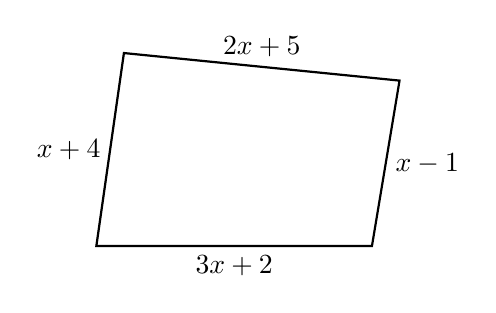
\begin{tikzpicture}[scale=0.7]
  \draw[thick] (0,0) -- (5,0) -- (5.5,3) -- (0.5,3.5) -- cycle;
  \node[below] at (2.5,0) {$3x + 2$};
  \node[right] at (5.25,1.5) {$x - 1$};
  \node[above] at (3,3.25) {$2x + 5$};
  \node[left] at (0.25,1.75) {$x + 4$};
\end{tikzpicture}
\end{center}
\end{questionText}
\choiceA{$7x + 10$}
\choiceB{$6x + 10$}
\choiceC{$7x + 12$}
\choiceD{$6x + 2$}
\correctAnswer{A}
\explanation{Add all sides: $(3x + 2) + (x - 1) + (2x + 5) + (x + 4)$. $x$-terms: $3x + x + 2x + x = 7x$. Constants: $2 - 1 + 5 + 4 = 10$. Perimeter: $7x + 10$.}
\end{practiceQuestion}

\begin{practiceQuestion}{4-5-q24}{gmc}
\begin{questionText}
The bar diagram below represents a subtraction problem. What is the simplified result?

\begin{center}
\begin{tikzpicture}[scale=0.55]
  % Top bar
  \draw[thick, fill=funBlue!20] (0,2) rectangle (8,3.5);
  \node at (4,2.75) {$6x + 10$};
  % Bottom bar (being subtracted)
  \draw[thick, fill=funOrange!20] (0,0) rectangle (5,1.5);
  \node at (2.5,0.75) {$4x + 3$};
  % Minus sign
  \node[font=\Large] at (-1,1.5) {$-$};
  % Equals
  \node[font=\Large] at (9,1.5) {$=$};
  % Result bar
  \draw[thick, fill=funGreen!20] (10,0.75) rectangle (14,2.25);
  \node at (12,1.5) {$?$};
\end{tikzpicture}
\end{center}
\end{questionText}
\choiceA{$10x + 13$}
\choiceB{$2x + 13$}
\choiceC{$2x + 7$}
\choiceD{$10x + 7$}
\correctAnswer{C}
\explanation{$(6x + 10) - (4x + 3) = 6x + 10 - 4x - 3 = 2x + 7$.}
\end{practiceQuestion}

% --- Graphical Short Answer Questions (3) ---

\begin{practiceQuestion}{4-5-q25}{gsa}
\begin{questionText}
The L-shaped figure below is made of two rectangles. Write a simplified expression for the total perimeter.

\begin{center}
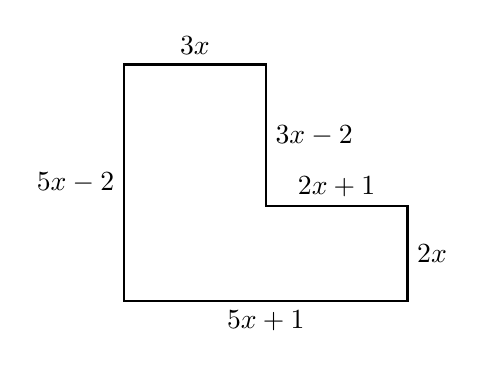
\begin{tikzpicture}[scale=0.6]
  % L-shape
  \draw[thick] (0,0) -- (6,0) -- (6,2) -- (3,2) -- (3,5) -- (0,5) -- cycle;
  % Dimensions
  \node[below] at (3,0) {$5x + 1$};
  \node[right] at (6,1) {$2x$};
  \node[above] at (4.5,2) {$2x + 1$};
  \node[right] at (3,3.5) {$3x - 2$};
  \node[above] at (1.5,5) {$3x$};
  \node[left] at (0,2.5) {$5x - 2$};
\end{tikzpicture}
\end{center}
\end{questionText}
\correctAnswer{$20x - 2$}
\explanation{Perimeter $= (5x + 1) + 2x + (2x + 1) + (3x - 2) + 3x + (5x - 2)$. $x$-terms: $5x + 2x + 2x + 3x + 3x + 5x = 20x$. Constants: $1 + 0 + 1 - 2 + 0 - 2 = -2$. Result: $20x - 2$.}
\end{practiceQuestion}

\begin{practiceQuestion}{4-5-q26}{gsa}
\begin{questionText}
The table shows Noah's earnings and expenses over two weeks. Write a simplified expression for his total profit.

\begin{center}
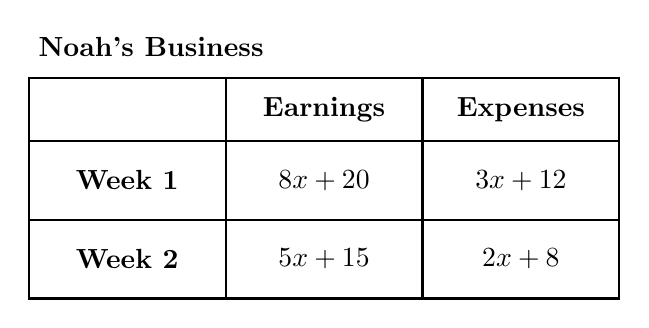
\begin{tikzpicture}
\node[anchor=west] at (0,3.2) {\textbf{Noah's Business}};
\draw[thick] (0,0) rectangle (7.5,2.8);
\draw[thick] (0,2) -- (7.5,2);
\draw[thick] (0,1) -- (7.5,1);
\draw[thick] (2.5,0) -- (2.5,2.8);
\draw[thick] (5,0) -- (5,2.8);
\node at (1.25,2.4) {};
\node at (3.75,2.4) {\textbf{Earnings}};
\node at (6.25,2.4) {\textbf{Expenses}};
\node at (1.25,1.5) {\textbf{Week 1}};
\node at (3.75,1.5) {$8x + 20$};
\node at (6.25,1.5) {$3x + 12$};
\node at (1.25,0.5) {\textbf{Week 2}};
\node at (3.75,0.5) {$5x + 15$};
\node at (6.25,0.5) {$2x + 8$};
\end{tikzpicture}
\end{center}
\end{questionText}
\correctAnswer{$8x + 15$}
\explanation{Total earnings: $(8x + 20) + (5x + 15) = 13x + 35$. Total expenses: $(3x + 12) + (2x + 8) = 5x + 20$. Profit $= (13x + 35) - (5x + 20) = 13x + 35 - 5x - 20 = 8x + 15$.}
\end{practiceQuestion}

\begin{practiceQuestion}{4-5-q27}{gsa}
\begin{questionText}
The two scales below show the weight of containers. The first scale reads $(9x + 5)$ units and the second scale reads $(4x + 12)$ units. Write a simplified expression for how much heavier the first set is than the second.

\begin{center}
\begin{tikzpicture}[scale=0.6]
  % Scale 1
  \draw[thick] (0,0) -- (5,0);
  \draw[thick] (2.5,0) -- (2.5,-0.5);
  \draw[thick] (1.5,-0.5) -- (3.5,-0.5);
  \draw[thick, fill=funBlue!20] (0.5,0) rectangle (4.5,1.5);
  \node at (2.5,0.75) {$9x + 5$};
  \node[below] at (2.5,-1) {Scale 1};
  % Scale 2
  \draw[thick] (8,0) -- (13,0);
  \draw[thick] (10.5,0) -- (10.5,-0.5);
  \draw[thick] (9.5,-0.5) -- (11.5,-0.5);
  \draw[thick, fill=funGreen!20] (8.5,0) rectangle (12.5,1.5);
  \node at (10.5,0.75) {$4x + 12$};
  \node[below] at (10.5,-1) {Scale 2};
\end{tikzpicture}
\end{center}
\end{questionText}
\correctAnswer{$5x - 7$}
\explanation{Difference $= (9x + 5) - (4x + 12) = 9x + 5 - 4x - 12 = 5x - 7$.}
\end{practiceQuestion}
